\documentclass[english]{article}
\usepackage[T1]{fontenc}
\usepackage[latin9]{inputenc}
\usepackage{url}
\usepackage{graphicx}
\usepackage[authoryear]{natbib}
\usepackage{babel}
\usepackage{fullpage}
\usepackage{hyperref}
\newcommand{\pkg}[1]{{\fontseries{b}\selectfont #1}}

\begin{document}

\title{MissingDataGUI: A Graphical User Interface for Exploring Missing Values in Data}


\author{Xiaoyue Cheng, Heike Hofmann, Dianne Cook \\ Department of Statistics, Iowa State University}

\maketitle
\begin{abstract}
Missing values are common in data, and usually require attention in order to conduct statistical analysis.  One of the first steps is to explore the structure of the missing values, and how missingness relates to the other collected variables.  This article describes an R package, that provides a graphical user interface (GUI) designed to help explore the missing data structure and examine the results of different imputation methods. The GUI provides numerical and graphical summaries conditional on missingness, and includes  imputations using fixed values, multiple imputations and nearest neighbors.

\textbf{Keywords:} imputation, exploratory data analysis, statistical graphics, visualization.
\end{abstract}

\section{Introduction}

Missing values are a very common problem affecting data analysis. Many imputation methods are developed but little has been done for exploring the missing value structure visually.  Most plotting methods handle missing values by simply removing the incomplete records with or without a warning, especially when the data are continuous. Most statistical functions provide a limited list of handling missing values, such as delete all cases with missing, delete pairwise or on single variables only.

The issue is that in order to decide what to do with the missing values before analyzing the data, we need to understand what the distribution of the missing values is, and how the missingness depends on the other collected variables. Some R packages, \pkg{norm} \citep{norm}, \pkg{Hmisc} \citep{hmisc}, which have some routines for summarizing the number of missing by variable, and by case, in preparation for imputing the missing values. To understand the distribution of missings vs not missings we need to make plots of the data.

Some existing work describing the types of plots needed to explore missing data, and implementations, can be found in \citet{unwin1996interactive} and \citet{swayne1998missing}. Both use interactive graphics to help with the exploration.  MANET implements the methods described in \citet{unwin1996interactive}. It presents the segmented barcharts of missing vs not missing for each variable. Because it has multiple plot types, histograms, scatterplots, mosaic plots, MANET encourages the user to select cases that are missing on any variable which highlights these cases in other plots enabling the user to explore the missing status dependence in the distributions of the complete cases of other variables.  XGobi, which implements the ideas described in \citet{swayne1998missing} provides more real-valued data tools. It creates a shadow matrix of the original data where entries are 0 (complete) or 1 (missing value). This additional data structure allows the user to explore the multivariate pattern of missing values, and to explore dependence between missing value status and distribution of the complete cases. Again, linked brushing is used, and rudimentary imputation methods are available in GGobi \citep{STLBC03}.

This current work describes a new package for R, \pkg{MissingDataGUI}, which allows the exploration of missing values structure, and results of imputation, using static graphics and numerical summaries. A graphical user interface (GUI) makes is accessible to novice users. This work builds on the ideas developed in \citet{unwin1996interactive} and \citet{swayne1998missing}. This package utilizes routines in \pkg{Hmisc} \citep{hmisc}, \pkg{norm} \citep{norm} for some imputation methods. The paper is structured as follows. Section 2 explains what is done in GUI and why. Section 3 describes the design of GUI and gives an example. The last section discusses future work.

\section{Functionality}

\begin{center}
%
\begin{figure}[h]
\begin{centering}
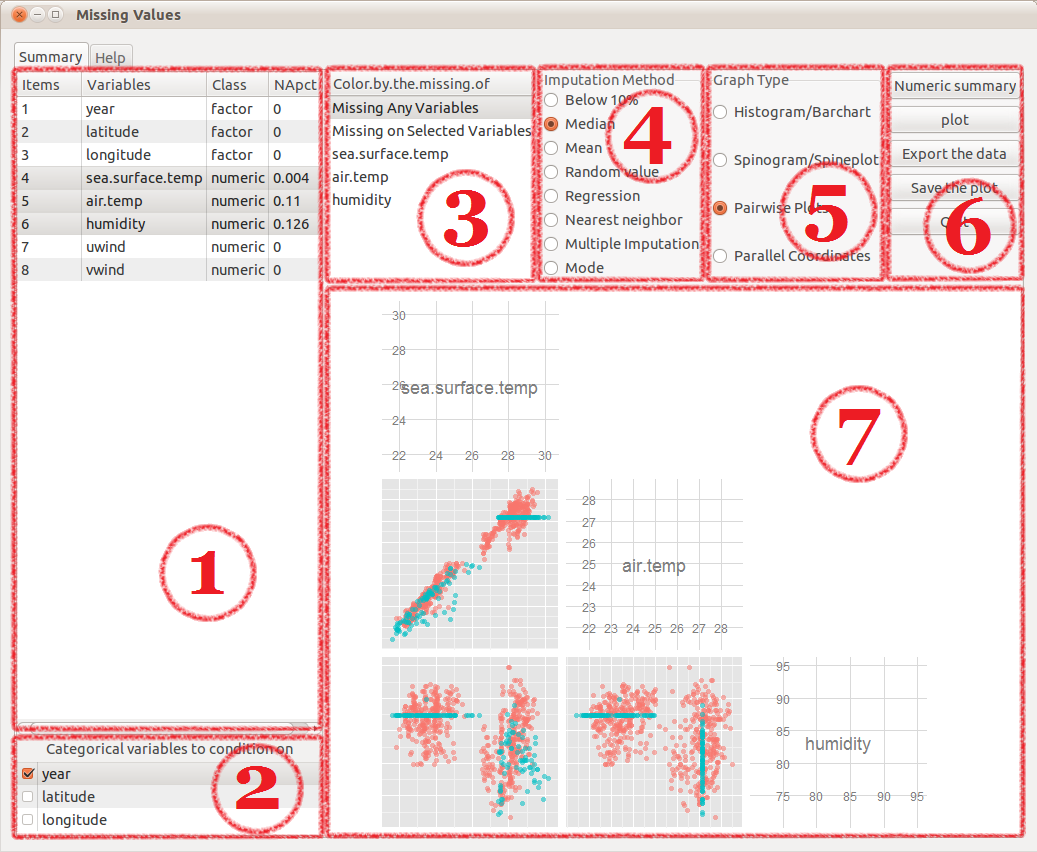
\includegraphics[width=.9\textwidth]{fig1-1-0}
\par\end{centering}

\caption{Overview of the missing data GUI. Region 1 contains the list of variables, variable type, and summary of missings on that variable. Region 2 has a list of the categorical variables that can be used to conditionally impute values. Region 3 lists the variables with missing values to enable coloring by different types of missingness in the plots. Region 4 contains a radio button selection of imputation methods. Region 5 has several plot type selections, and section 6 allows selecting numeric or graphical summaries and some output routines. The summaries are displayed in the region 7.}
\label{fig: missingGUI}
\end{figure}

\par\end{center}


\subsection{Overview of missing data GUI}

The missing data GUI looks as Figure \ref{fig: missingGUI}. All variables with the classes and the percentages of NA's are listed on the top left (area 1). The categorical variable is shown on the bottom left as the condition (area 2). The variables having missing values are displayed under ``Color.by.the.missing.of'' on the top center (area 3). The first row ``Missing Any Variables'' in the list means whether the case having missing values in any variables, and the second row ``Missing on Selected Variables'' means whether the case having missings in those variables selected in area 1. ``Imputation Method'' (area 4) and ``Graph Type'' (area 5) are two radios interpreted in section 2.2 and 2.3. Five buttons on the top right (area 6) are: ``Numeric summary'' which will create a window like Figure \ref{fig: num-summry}; ``plot'' which produces the plots in the graphics device on the bottom right of GUI (area 7); ``Export the data'' which will save the imputed data into a data file; ``Save the plot'' which could save the plot in area 7 to a png file; ``Quit'' which will destroy the main GUI window and the numeric summary window.

\subsection{Summary of missing values}

To investigate missingness in a data set, numerical summaries of the missings are initially calculated, as shown in Figure \ref{fig: num-summry}. The information at the top of the window contains the percent of the values that are missing, along with the percent of variables that contain missing values and the percent of the cases that have at least one missing value. Below this is a tabulation of the number of values missing per case - here at most 2 cases have 3 missing values, another 2 have 2 missing values, 167 cases have one missing value and there are 565 complete cases. In terms of percentages, 76.8\% of the cases are complete. This follows the style of the norm package for summarizing missingness.


\begin{center}
%
\begin{figure}[h]
\begin{centering}
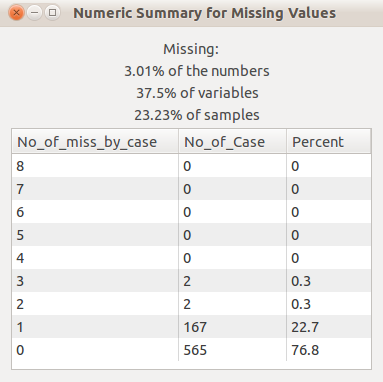
\includegraphics[width=0.4\textwidth]{Miss_fig2}
\par\end{centering}
\caption{A numerical summary of missing values in the data is shown in a pop-up window.  The percentage of missings by total number of data values, by variables and by cases, is shown at the top. This data has 8 variables and the missing values across variables is summarized in the lower table. No cases have more than 3 missing values.  76.8\% of cases are complete, 22.7\% of cases have one missing value, and only 4 cases have more than one missing values.}
\label{fig: num-summry}
\end{figure}

\par\end{center}

\subsection{Imputation}

A number of imputation methods are available in the package. The purpose of these is both for examining the dependence between missing or not missing and for producing a complete data set for later analysis.  The eight imputation methods available are: 
``Below 10\%'', ``Median'', ``Mean'', 
``Random value'', ``Regression'', ``Nearest neighbor'', 
``Multiple imputation'', ``Mode''. 
The first four, as well as ``Mode'', are imputations on individual variables, and the remainder  ``Regression'', ``Nearest neighbor'', and ``Multiple imputation'' are imputations on the joint distribution of two or more  variables.


\begin{center}
\begin{figure}[h]
\begin{centering}
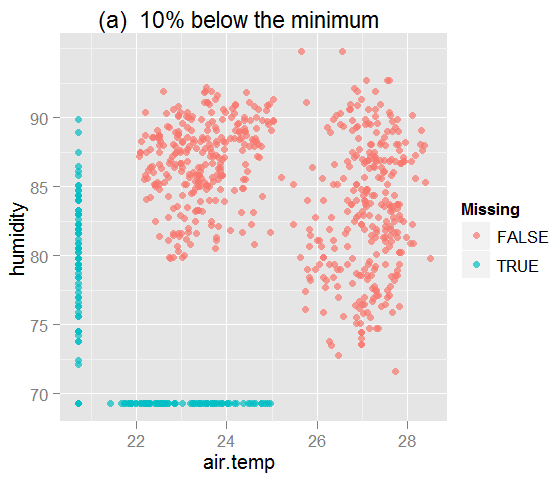
\includegraphics[width=0.45\textwidth]{fig3-1} 
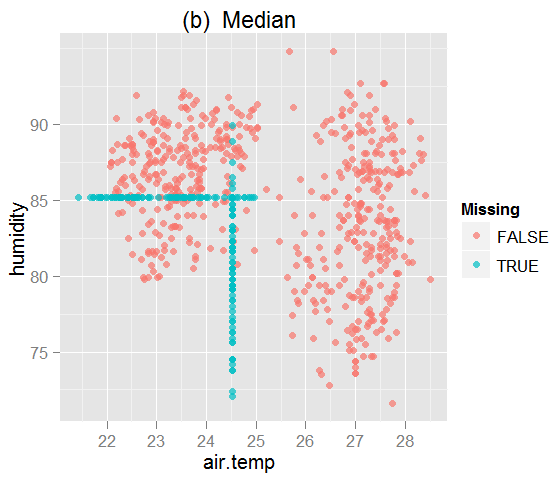
\includegraphics[width=0.45\textwidth]{fig3-2}
\par\end{centering}

\begin{centering}
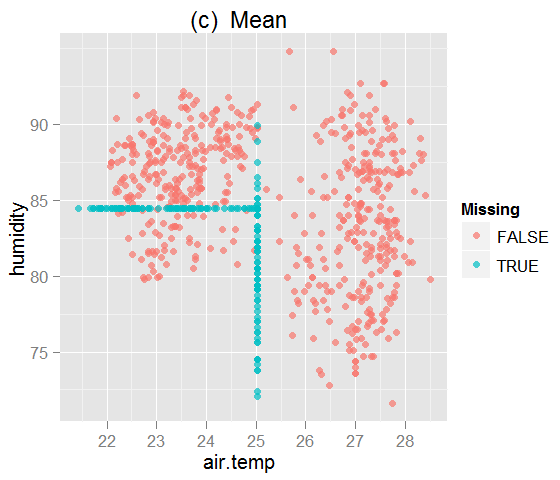
\includegraphics[width=0.45\textwidth]{fig3-3} 
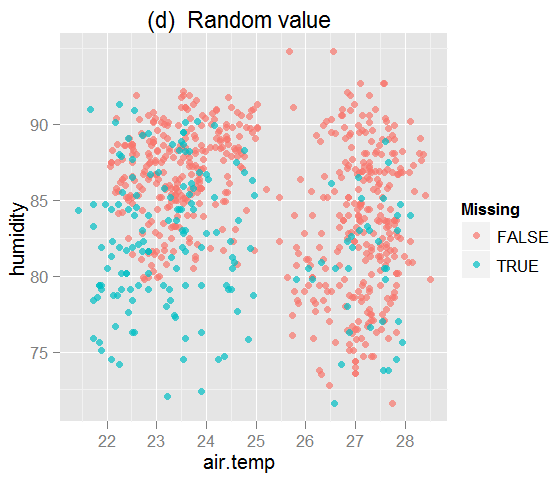
\includegraphics[width=0.45\textwidth]{fig3-4}
\par\end{centering}

\caption{\label{fig:univariate-imputation}Four panels of scatterplots displaying the results of different univariate imputations (cyan=missing, peach=not missing): (a) 10\% below the minimum (not strictly an imputation method, it is used more for displaying missings as part of a plot of complete cases); (b) median of each variable; (c) mean of each variable; (d) random selection from the complete cases. }

\end{figure}
\par\end{center}

\subsubsection{Univariate imputations}

The simplest example is setting the missing values to 10\% below the minimum of each variable. The purpose of this approach is to include the missing values in a plot in a place which they can be distinguished from the complete values. In a scatterplot, all missing values will lie along a vertical line on the left or a horizontal line on the bottom of the display (Figure \ref{fig:univariate-imputation} (a)). In the histogram, missing values will be in a bar to the left of other data values. And in the parallel coordinates plot, the missing values are at the bottom of each axis.

Using the median, mean or mode of the complete cases on a variables is a common way to impute missing values. The median and mean are used for the continuous variables, and mode is used for categorical variables. Using the mean for imputed values  leaves the variable mean as that of the complete cases. For a categorical variable, using the mode imputes the missing as the most common category. To examine the location of these imputed values with the complete cases in plots of the data, points and bars are colored according to the missing value status of the case. Figure \ref{fig:univariate-imputation} (b) and (c) give an example of the imputation by median and mean for real-valued variables.

Choosing a ``random value''  will randomly select from the complete cases on a variable to impute the missing value, as shown in Figure \ref{fig:univariate-imputation} (d).

Because these imputation methods operate separately on each variable, the resulting data have different covariance and correlation estimates. In some circumstances this may still enable reasonable further analysis.

\subsubsection{Multiple imputations}

These methods will conduct imputation on the joint distribution of the selected variables. 

The ``regression'' method uses function \texttt{aregImpute} from package \pkg{Hmisc}. The function provides multiple imputation using additive regression, bootstrapping, and predictive mean matching\citep{hmisc}. The ``multiple Imputation'' method uses functions from package \pkg{norm}. The process draws samples from a multivariate normal model with estimated parameters\citep{norm}, so it requires all of the selected variables to be numeric (at least integers).

The ``nearest neighbor'' method replaces a missing value with the mean of its 5 nearest neighbors by squared Euclidean distance. If there are ties in the distance ranking, only the first five points are used, regardless to the tie. This method requires at least one case to be complete, and no character variables. If there are more than one but less than five complete cases, the mean of them will be imputed. If none of the cases are complete, then the median of each variable is returned. The algorithm and code is described in the Appendix.

The strength of the above methods includes 1) they incorporate covariace information when calculating imputed values, and  2) ``regression'' and ``nearest neighbor'' can accommodate both continuous and categorical data.

\begin{center}
%
\begin{figure}[h]
\begin{centering}
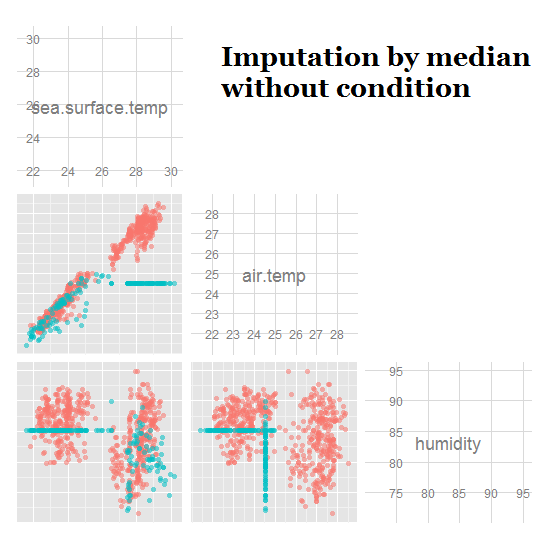
\includegraphics[width=.48\textwidth]{fig4-1}
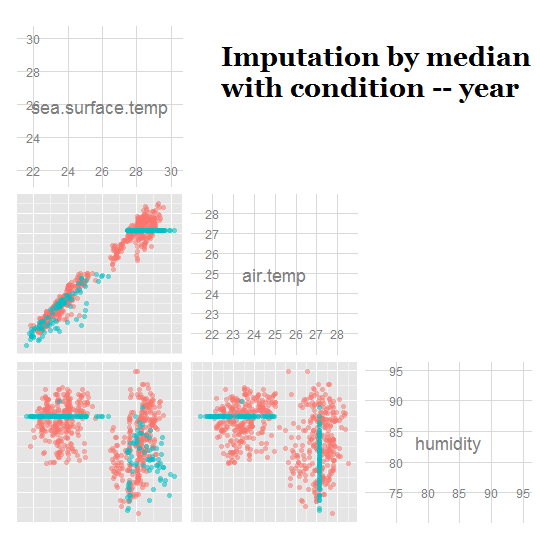
\includegraphics[width=.48\textwidth]{fig4-2}
\par\end{centering}

\caption{\label{fig: condition}{Comparison between imputations
with and without conditions. The left panel is imputation by median
without condition and the right one is conditioned on year. In the left plot you can see that the imputed values fall between the two clusters, at the overall median, but when the imputation is conditioned on year (right plot) the imputed values are now better placed into the two clusters in the data.}}

\end{figure}

\par\end{center}

\subsubsection{Condition on the categorical variables}

When the variables of interest are bimodal or multi-modal, using the center statistics like mean or median as the imputations is inadequate because the center can not reflect the distribution. In many situations, the modalities arise from the mixture of groups. Hence, a better imputation method is to use the group means or medians instead of the population mean or median.

The extension of this idea produces the widget named ``categorical variables to condition on''. All categorical variables are listed with checkboxes. The variables checked will partition the data into grids and then the imputation method is implemented in each group of data. The procedure is as computing based on the conditional model given the category. However, the condition is invalid when the imputation method is ``Below 10\%'', since the aim of ``Below 10\%'' is only displaying the missings away from the non-missings, but giving the condition will mix the points again.

The role of conditions in the imputation is revealed in Figure \ref{fig: condition}. Without the condition, the imputations may locate far away from the distribution of values (Figure \ref{fig: condition} left). But the group median is much better in the plots (Figure \ref{fig: condition} right).

\subsection{Plot types}

\begin{center}
%
\begin{figure}[h]
\begin{centering}
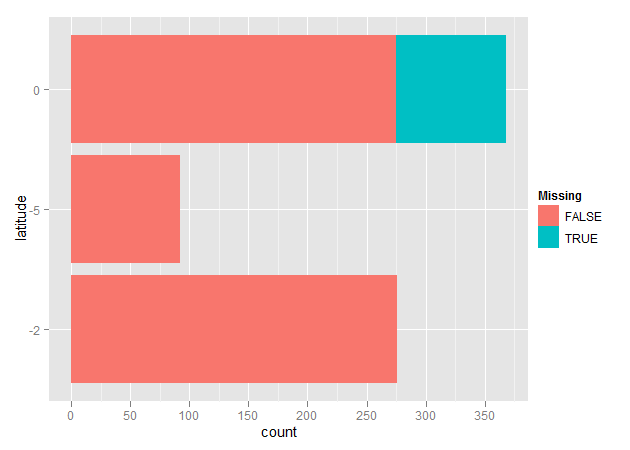
\includegraphics[width=.24\textwidth]{fig5-1-1}
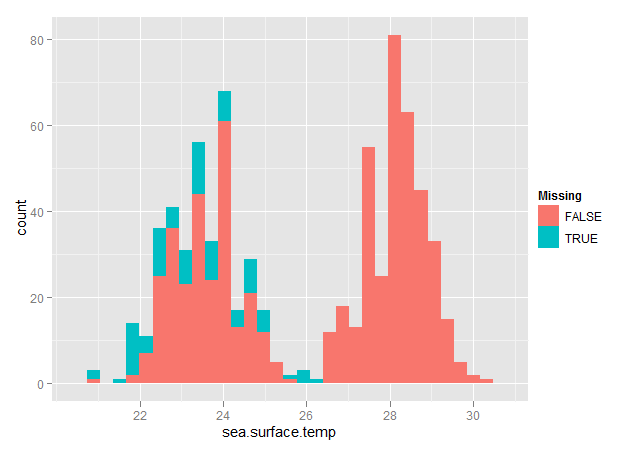
\includegraphics[width=.24\textwidth]{fig5-1-2}
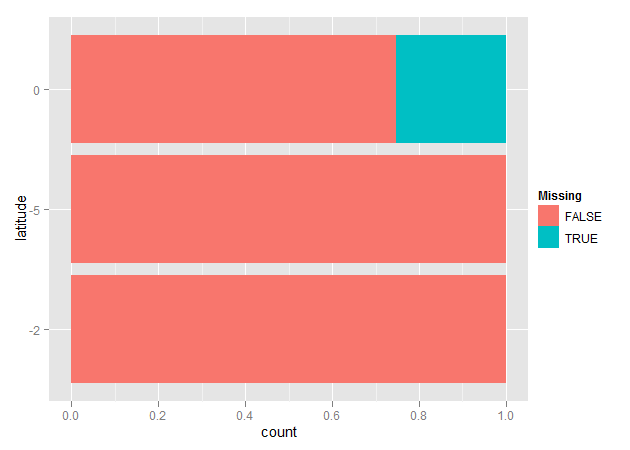
\includegraphics[width=.24\textwidth]{fig5-1-3}
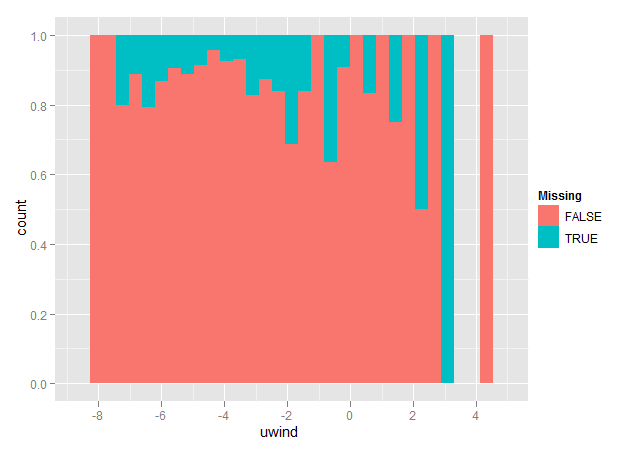
\includegraphics[width=.24\textwidth]{fig5-1-4}
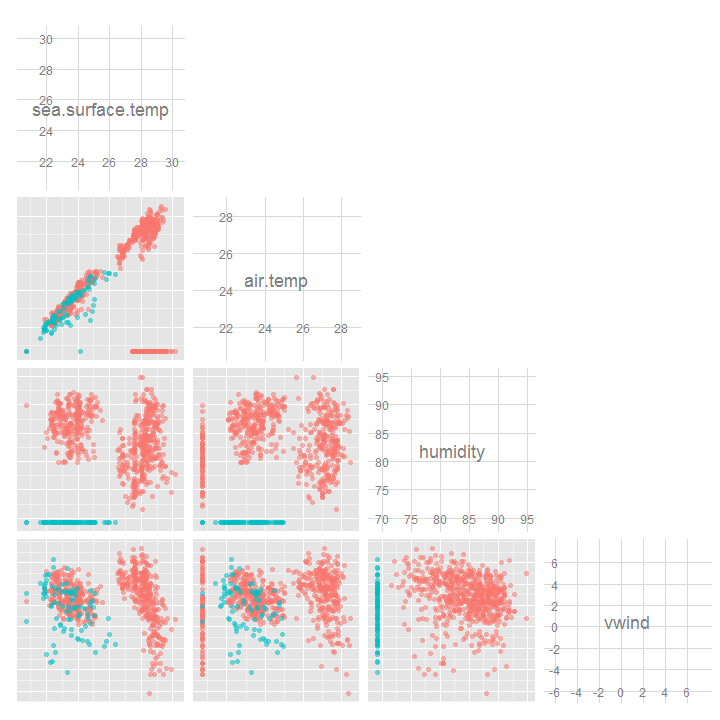
\includegraphics[width=.39\textwidth]{fig5-2-1}
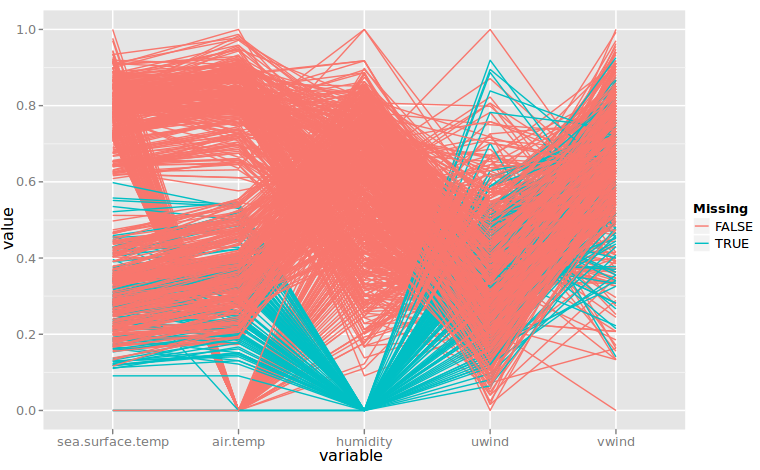
\includegraphics[width=.60\textwidth]{fig5-2-2}
\par\end{centering}

\caption{\label{fig:graphtypes}{Results for four types of graphs.
The left two graphs on the first row are a barchart and a histogram; the right two on the first row are a spineplot and a spinogram. The left panel on the second row presents the pairwise plots, and the right on the second row is the parallel coordinates plot. All the plots above use ``below 10\%'' imputation and color by the missing of one variable - humidity. }}

\end{figure}

\par\end{center}

Four types of graphs are available in the GUI: histogram (for continuous data)/barchart (for discrete data), spinogram/spineplot, pairwise plots and parallel coordinates plot. For all those graphs, color represents missing or not missing of one or more variables with missing values. 

The histograms and barcharts are shown one by one for all the variables selected. When the missing values and the complete values share one bar, the bar is cut to two parts, and the ratio of two heights is equal to the ratio of missing and non-missing values in that bar. Besides, the histogram is laid vertically while barchart is horizontal, which will clearly differ the continuous and discrete data.

The spinograms and spineplots are presented similar as histograms. Each bar has the same height, but is partitioned by two colors which represent the missing and non-missing values. The ratio of two heights is equal to the ratio of missings and non-missings too. Both histogram/barchart and spinogram/spineplot are based on the package \pkg{ggplot2} \citep{ggplot2}.

Pairwise plots are drawn by the function \texttt{ggpairs} of package \pkg{GGally} \citep{ggally}. The pairwise plots are in the lower triangular while the variable names and scales lay in the diagonal. For the continuous variables the pairwise plots are scatterplots and for the categorical variables they are ratio plots. The combo of continuous and categorical variables is side-by-side boxplots of missing and non-missing values for each category. Limited by the room of the graphics device in the main window, the pairwise plots cannot contain too many variables. The upper number of variables is set to be 5 and the lower is 2, obviously.

Parallel coordinates plot is in the use of function \texttt{ggpcp} from package \pkg{ggplot2} \citep{ggplot2}.

Figure \ref{fig:graphtypes} displays the different types of graphs in the missing data GUI. The color is based on whether missing in humidity or not. It is clear to see the location of incomplete cases at other covariates. Categorical covariates could also be displayed as boxplots or ratio plots in pairwise plots. 

\subsection{Design Issues}


%\subsubsection{Maps to items in GUIs}

The missing data GUI is designed in one window. The list of variables, the radio for imputation methods, the checkbox group for the conditional variables, and the graphics device, except for the numeric summary, are all in the same window. An appropriate layout makes the widgets look not crowded, but very easy to maintain. 

\begin{center}
%
\begin{figure}[h]
\begin{centering}
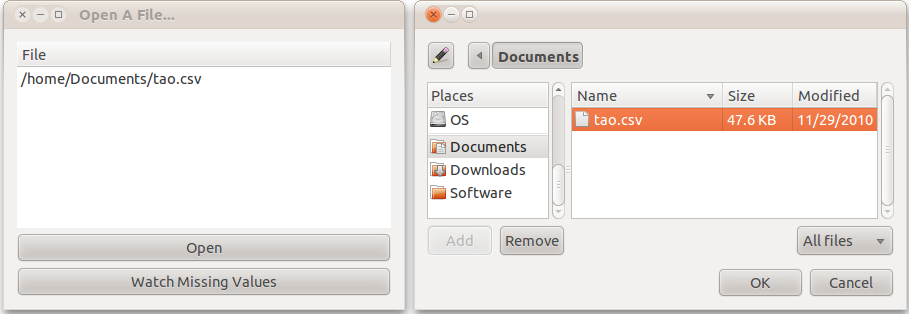
\includegraphics[width=0.9\textwidth]{Miss_fig6}
\par\end{centering}

\caption{\label{fig: import}{The data import GUI, with file selector, which is called by the ``open'' button. You could list more than one file in the data import GUI, but are only able to select one data set to check the missings. The first file is automatically chosen if none of the data sets is focused when clicking ``Watching Missing Values'' button. }}

\end{figure}

\par\end{center}

\subsection{Read in data}

The data can be read in as either a data frame or from a file. To read in a data frame, the data is input as a parameter to the \texttt{MissingDataGUI()} function.  An advantage is that the type of variables (factor, numeric, ...) as characterized by R are used. This is the preferred approach.

It is also possible to read from a file.  If the \texttt{MissingDataGUI()} is called without a data frame argument, data import GUI is called (Figure \ref{fig: import}).  The ``Open'' button is for choosing files and the ``Watch Missing Values'' buttons opens the missing data GUI. The file should be a ``comma separated value'' file. Only one data set can be imported at any time.

Two data sets are provided with the package, \texttt{tao}, used in the Example section, and \texttt{brfss}. The latter data set is a subset of the 2009 survey from the Behavioral Risk Factor Surveillance System (BRFSS), an ongoing data collection program designed to measure behavioral risk factors for the adult population (18 years of age or older) living in households. The website for this program is \url{http://www.cdc.gov/BRFSS/index.htm}.


\begin{center}
%
\begin{figure}[h]
\begin{centering}
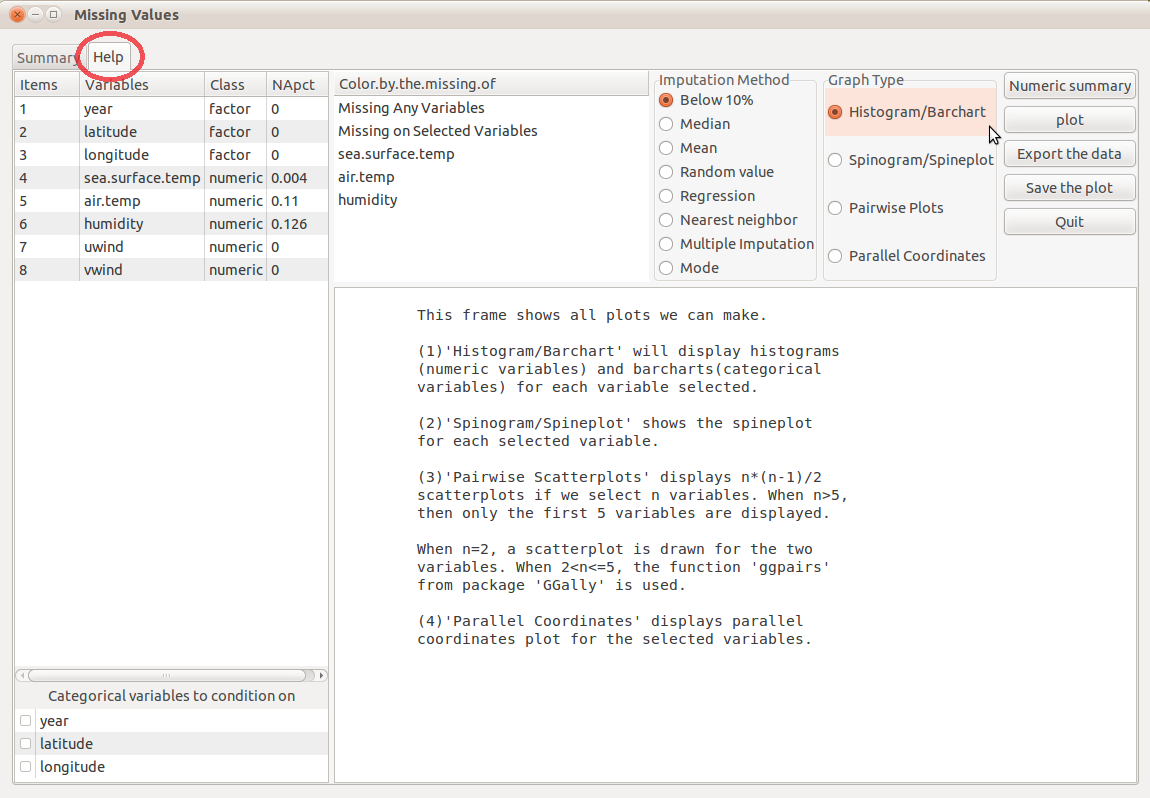
\includegraphics[width=0.9\textwidth]{Miss_fig7}
\par\end{centering}

\caption{The help tab of missing data GUI. Mousing over any part of the GUI or clicking the radio/checkbox items will pop up text explanations in the summary region. All the widgets have their detailed introduction for each item.}
\label{fig: missingGUI-help}
\end{figure}

\par\end{center}


\subsection{Help tab}

The help tab shown in Figure \ref{fig: missingGUI-help} has the same layout as the summary tab. The only difference is that the graphics device is replaced by the help document of each widget.

\begin{center}
%
\begin{figure}[h]
\begin{centering}
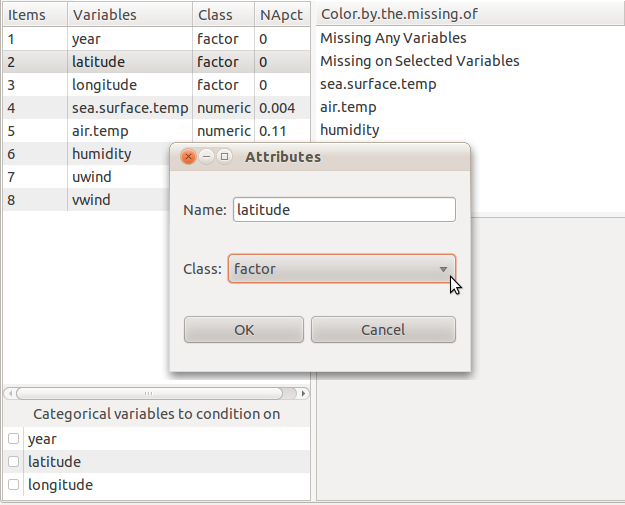
\includegraphics[width=0.6\textwidth]{Miss_fig8}
\par\end{centering}

\caption{The attributes list for variable selection is interactive. The name can be edited, and the class could be changed to one of the four classes: integer, numeric, factor, and character. When a numeric variable is changed to a categorical variable, the condtions will be updated.}
\label{fig: attributes}
\end{figure}

\par\end{center}

\subsection{Additional features of the GUI}
In this part some additional features of the missing data GUI are explained.
\begin{itemize}
\item Double clicking on any variables in the top left table will open an attributes window, as displayed in Figure \ref{fig: attributes}. When the class of a variable is changed from numeric or integer to factor or character, the variable will be automatically loaded into the checkbox group for conditions.
\item The color by variable selector allows text entry to find the variable.
%(Figure \ref{fig: colorby}). 
This feature is very useful when there are a lot 
of variables with missing values.
%\end{itemize}
%begin{center}
%
%\begin{figure}[h]
%\begin{centering}
%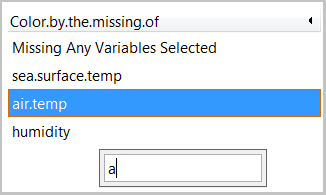
\includegraphics[width=0.4\textwidth]{colorby}
%\par\end{centering}
%\caption{The window of attributes for selecting variable to condition on.}
%\label{fig: colorby}
%\end{figure}

%\par\end{center}
\item The plots can be saved to file using the ``Save the plot'' button. It saves them in \texttt{png} format. All of the figures in the Example section were saved this way.
\item The imputed data can be saved by the ``Export the data'' button. Whether the exported data being imputed or not is indicated by the missing shadow matrix, which is also saved. 
%Figure \ref{fig: savefile} presents the interface for saving data.
\end{itemize}
%\begin{center}
%
%\begin{figure}[h]
%\begin{centering}
%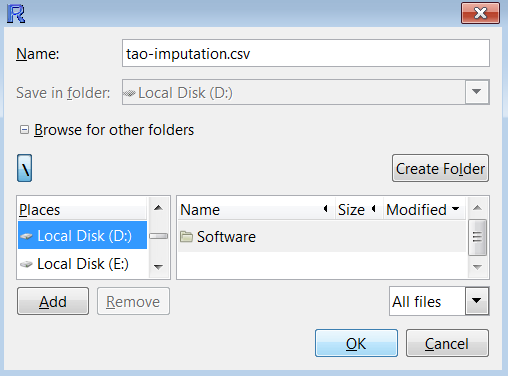
\includegraphics[width=0.5\textwidth]{save}
%\par\end{centering}

%\caption{The window for saving the imputed data set.} 
%\label{fig: savefile}
%\end{figure}

%\par\end{center}

\section{Example}


\subsection{Data}
The data is from the Tropical Atmosphere Ocean project (TAO) \citep{tao}. The TAO array consists of approximately 70 moorings in the Tropical Pacific Ocean, telemetering oceanographic and meteorologic al data to shore in real-time via the Argos satellite system. A subset of data from 6 moorings in 1993 and 1997 is used for the example. The data has 8 variables (year, latitude, longitude, sea surface temperature, air temperature, humidity, uwind and vwind) and 736 observations. This subset is provided by \citet{CS07}. Open the data using the commands:

\begin{verbatim}
> library(MissingDataGUI)
> data(tao)
> MissingDataGUI(tao)
\end{verbatim}

The numeric summary of all 8 variables in this data is shown in Figure \ref{fig: num-summry}.

%The access
%to data is as Figure \ref{fig: import} and by clicking the button
%``Watch Missing Values'' in the data import
%GUI we will get Figure \ref{fig: missingGUI} without activating the
%graphics device. 

\begin{figure*}[htp]
\centerline{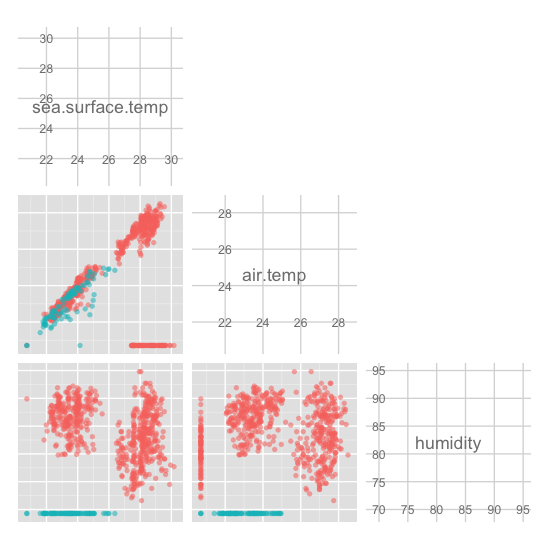
\includegraphics[width=0.49\textwidth]{tao1_pairwise.png}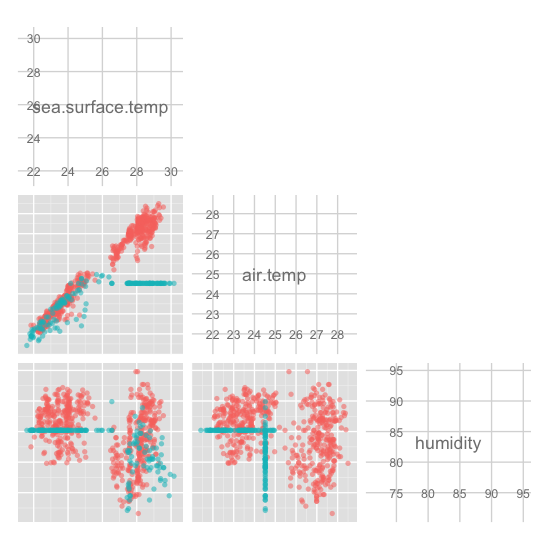
\includegraphics[width=0.49\textwidth]{tao2_pairwise.png}}
\caption{(Left) Exploring the effect missingness of humidity (cyan) on sea and air temperature. Missings on humidity occur at the lower temperature values, suggesting a dependence relationship. Missing values are not missing at random. (Right) Exploring imputation methods. Imputation using the medians is shown here. Values that have been imputed are shown as cyan. Median imputation introduces a cross structure to the point scatter, and the imputed values don't match the data well, for example the line of imputed values very apart from the complete cases in the plot of the tao temperature variables.}
\label{tao1}
\end{figure*}

\subsection{Exploring Missings}

Three of the 8 variables have missing values. First let's look at the distribution of missings on these variables. Figure \ref{tao1} (left) shows the pairwise plots of these three variables with missing values on humidity colored (cyan). Cases which are missing on humidity have  low values of sea and air temperature. This suggests a dependence pattern between humidity missingness and the temperature variables. Imputation methods that incorporate this dependence may be preferable.

Figure \ref{tao1} (right) shows the data imputed with median values (cyan). This imputation imposes a cross structure on the data, which doesn't match the shape of the complete cases very well. For example, there is a line of imputed values in the plot of air temperature vs sea surface temperature which is very separate from the rest of the complete cases. This imputation method doesn't work for this data!

%\begin{figure*}[p]
%\centerline{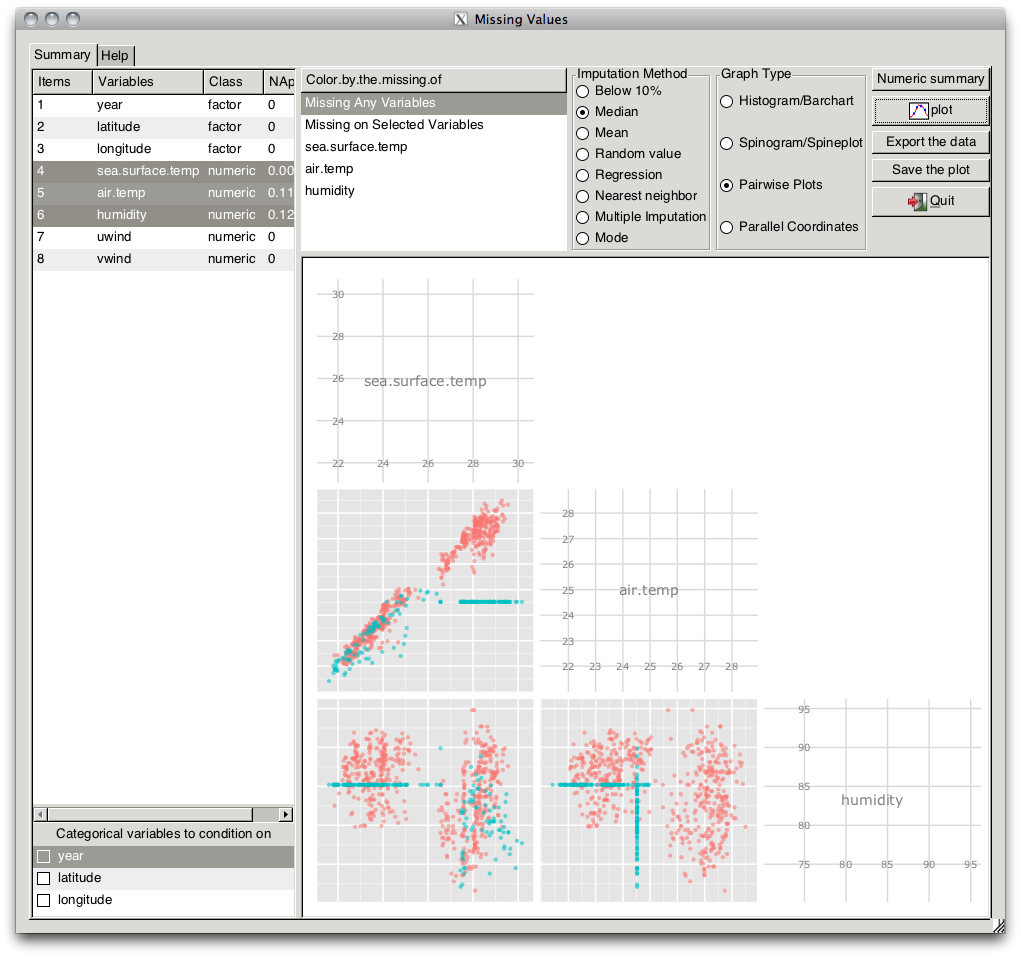
\includegraphics[width=0.9\textwidth]{tao2.png}}
%\caption{Exploring imputation methods. Imputation using the medians is shown here. Values that have been imputed are shown as cyan. Median imputation introduces a cross structure to the point scatter, and the imputed values don't match the data well, for example the line of imputed values very apart from the complete cases in the plot of the teo temperature variables.}
%\label{tao2}
%\end{figure*}

Figure \ref{tao3} (left) shows the data conditional imputing with median values (cyan) by year. This better matches the distribution of complete cases, although the imputed values still form bands in the scatterplot. This might be a problem because the variance estimation will be affected. 


\begin{figure*}[htp]
\centerline{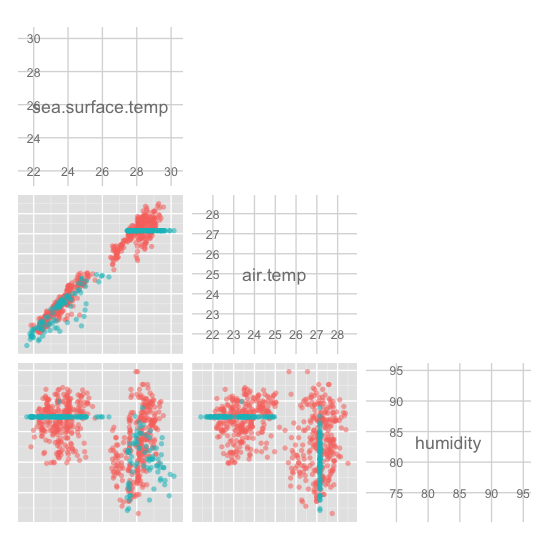
\includegraphics[width=0.49\textwidth]{tao3_pairwise.png}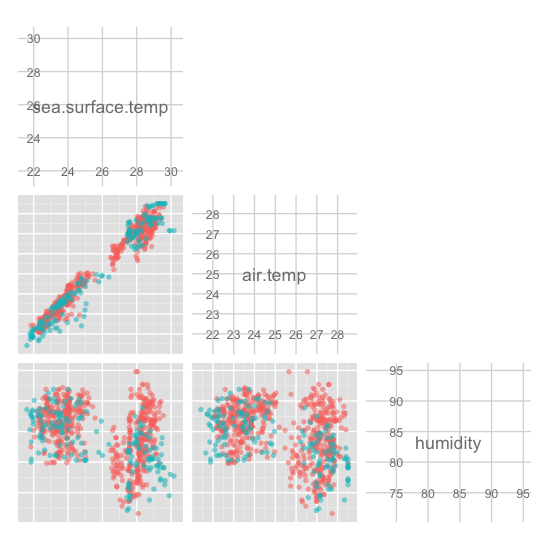
\includegraphics[width=0.49\textwidth]{tao5_pairwise.png}}
\caption{(Left) Imputation using the median conditional on year. Imputed values better match the complete cses, with the exception of the banding due to fixed median value. (Right) Imputation using the regression conditional on year. The distribution of imputed values fairly closely matches the distribution of complete cases.}
\label{tao3}
\end{figure*}

For this data, the better ways to impute the data would take the strong association between the variables into account. This suggests that regression, nearest neighbors, or multiple imputation might be the more desirable imputation methods. Figure \ref{tao3} (right) shows the results for regression-based imputation, conditional on year. The imputed values match the distribution of complete cases reasonably well. There are a few slight concerns: some of the imputed values have lower air temperature values than any of the complete cases, the spread of the imputed values is a little greater than the complete cases. But overall, this is probably as good as it is going to get with imputing the missings for this data set. It would be reasonable to export the imputed data for further analysis at this point.

%\begin{figure*}[p]
%\centerline{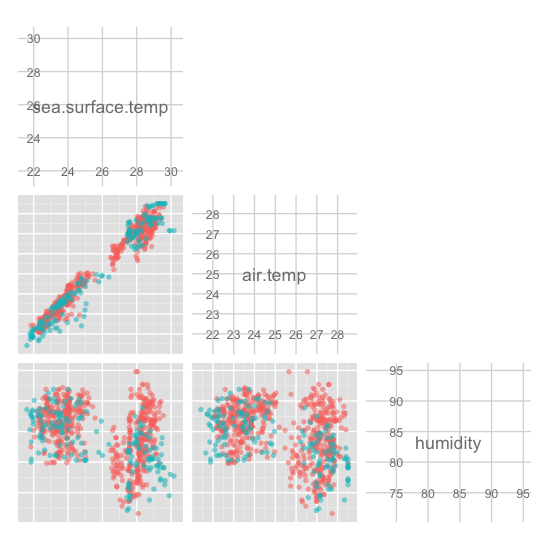
\includegraphics[width=0.45\textwidth]{tao5_pairwise.png}}
%\caption{Imputation using the regression conditional on year. The distribution of imputed values fairly closely matches the distribution of complete cases.}
%\label{tao4}
%\end{figure*}

\section{Discussion}

The main goal of this work is to make it possible to see the the missing data and the impact of various imputation methods. In the future interactive data visualization may make it possible to brush points in a plot to more completely explore missing structure as we can in GGobi and MANET.


\section*{Software}

This missing data GUI is written in R 2.13.0 \citep{r} and
based on the package gWidgets\citep{gwidgets} with the toolkit
RGtk2. 

Different platforms (Windows, Linux, Mac) will differ the appearance of the GUI slightly, but the functions are consistent.

\section*{Acknowledgements}

This work was partially supported by an unrestricted fellowship from Novartis, and National Science Research grant DMS0706949.

\bibliographystyle{apa}
\bibliography{missing}



\section*{Appendix: Code for Nearest Neighbor Imputation}

\begin{verbatim}
myNNdat = dat[complete.cases(dat),]
Missing_any = factor(apply(is.na(dat),1,any),levels=c(FALSE,TRUE))
for (i in which(Missing_any=='TRUE')){
    usecol = which(!is.na(dat[i,]))
    if (length(usecol)!=0){
        NNdat = myNNdat
        a = rbind(dat[i,], NNdat)[,usecol]
        NNdat$distance = dist(a)[1:nrow(NNdat)]
        k5NNdat = NNdat[order(NNdat$distance,decreasing=FALSE),][1:min(5,nrow(NNdat)),]
        if (nrow(k5NNdat)>1 & n-length(usecol)>1) {
            dat[,1:n][i,-usecol] = apply(k5NNdat[,1:n][,-usecol],2,mean)
        } else {
            if (nrow(k5NNdat)==1) {
                dat[,1:n][i,-usecol] = k5NNdat[,1:n][1,-usecol]
            } else {
                dat[,1:n][i,-usecol] = mean(k5NNdat[,1:n][,-usecol])
            }
        }
    } else {
        for (j in 1:n) {
            dat[i,j] = median(dat[,j], na.rm=TRUE)
        }
    }
}
\end{verbatim}

\end{document}
